% !TeX program = xelatex
% 编译：xelatex 07-连续信号卷积计算.tex（VS Code 的 LaTeX Workshop 会读上一行，自动用 xelatex）
% 来源：2022 浙江大学《信号与系统》胡浩基老师，连续信号卷积的计算（教材第 38--39 页例 2-1、例 2-2，第 78 页图 2-44，第 31 页 1-9）。
% 体例：先讲两种算法（直接代公式、图解法），再记两个方波卷积的结论，最后做综合例题和一道冲激尺度变换的易错题。
\documentclass[UTF8,a4paper,11pt]{ctexart}
\usepackage{amsmath,amssymb}
\usepackage{geometry}
\geometry{margin=2.4cm}
\usepackage{xcolor}
\usepackage{mdframed}
\usepackage{booktabs}
\usepackage{needspace}
\usepackage{array}
\usepackage{enumitem}
\usepackage{tikz}
\usetikzlibrary{arrows.meta,positioning,calc,patterns}
\usepackage{float}
\usepackage{fancyhdr}
% 页眉页脚清空，只在右下角保留页号（含首页）
\fancypagestyle{plain}{%
  \fancyhf{}%
  \fancyfoot[R]{\thepage}%
  \renewcommand{\headrulewidth}{0pt}%
  \renewcommand{\footrulewidth}{0pt}}
\usepackage[hidelinks,unicode,bookmarksnumbered,bookmarksopen=true,bookmarksopenlevel=2,pdftitle={连续信号卷积计算}]{hyperref}
\usepackage{bookmark}% XeTeX 下 hyperref 自带的大纲不生效，用 bookmark 宏包生成 PDF 书签（需编译两遍）

\setCJKmainfont{Songti SC}[BoldFont={Songti SC Bold}]
\setCJKsansfont{PingFang SC}

\newmdenv[backgroundcolor=blue!4,linecolor=blue!50!black,linewidth=1pt,innertopmargin=6pt,innerbottommargin=6pt]{rememberbox}
\newenvironment{remember}{\begin{rememberbox}\textbf{重点}\par\smallskip}{\end{rememberbox}}
\newmdenv[backgroundcolor=yellow!8,linecolor=orange!70!black,linewidth=1pt,innertopmargin=6pt,innerbottommargin=6pt]{notebox}
\newenvironment{note}{\begin{notebox}\textbf{说明}\par\smallskip}{\end{notebox}}

% ---------------------------------------------------------------- 画图用的小宏
% 坐标轴：\taxes[自变量名]{横轴起点}{横轴终点}{纵轴顶端}{纵轴底端}。原点标 0（放在左下，避开纵轴）。
\newcommand{\taxes}[5][t]{%
  \draw[->] (#2,0) -- (#3,0) node[right,font=\scriptsize] {$#1$};
  \draw[->] (0,#5) -- (0,#4);
  \node[anchor=north east,font=\tiny,gray!60!black,inner sep=1pt] at (0,-0.02) {$0$};}
% 横轴刻度 \xt{位置}{标签}（标在轴下方）、\xtu{位置}{标签}（标在轴上方，轴下方有曲线时用）、纵轴刻度 \yt{位置}{标签}：刻度线 + 白底数字。
\newcommand{\xt}[2]{\draw (#1,0) -- (#1,-0.1) node[anchor=north,font=\tiny,gray!60!black,fill=white,inner sep=0.6pt] {$#2$};}
\newcommand{\xtu}[2]{\draw (#1,0) -- (#1,0.1) node[anchor=south,font=\tiny,gray!60!black,fill=white,inner sep=0.6pt] {$#2$};}
\newcommand{\yt}[2]{\draw (0,#1) -- (-0.1,#1) node[anchor=east,font=\tiny,gray!60!black,fill=white,inner sep=0.6pt] {$#2$};}
% 冲激箭头 \imp{位置}{画出的高度}{强度标签}
\newcommand{\imp}[3]{\draw[->,ultra thick,red!70!black] (#1,0) -- (#1,#2);
  \node[anchor=south,font=\tiny,red!70!black,inner sep=1pt] at (#1,#2) {#3};}
% 两个图之间的运算符号
\newcommand{\opsym}[3]{\node[font=\Large] at (#1,#2) {#3};}
\tikzset{>=stealth,
  sig/.style={thick,blue!60!black},
  res/.style={thick,red!70!black},
  out/.style={thick,green!45!black}}

% ---------------------------------------------------------------- 标题层级
\definecolor{secblue}{RGB}{31,78,121}
\definecolor{exorange}{RGB}{190,90,10}
\definecolor{ptteal}{RGB}{0,110,110}
\ctexset{
  section={format=\raggedright\Large\bfseries\color{secblue},
           beforeskip=3.2ex plus 1ex minus .5ex, afterskip=1.4ex,
           aftertitle={\par\nobreak\vspace{-1.1ex}\noindent\textcolor{secblue}{\rule{\linewidth}{0.8pt}}\par\nobreak\vspace{0.6ex}}},
  subsection={format=\raggedright\large\bfseries\color{secblue},
              beforeskip=2.4ex plus .8ex minus .4ex, afterskip=1.0ex}
}
% 例题标题：\example{标题}{结论}{附注}，附注一般留空。左边橙色实心「例 n」，右边结论标签；同时进 PDF 大纲（第 3 级）。
\newcounter{ex}[section]
\newcommand{\example}[3]{%
  \refstepcounter{ex}\phantomsection
  \addcontentsline{toc}{subsubsection}{例 \theex\ #1（#2）}%
  \par\addvspace{1.6ex}\noindent
  {\setlength{\fboxsep}{3pt}%
   \colorbox{exorange}{\textcolor{white}{\textbf{例~\theex}}}\ %
   \textcolor{exorange}{\textbf{#1}}\ {\footnotesize\textcolor{gray!70!black}{#3}}%
   \hfill\colorbox{exorange!12}{\small\textcolor{exorange}{#2}}\par}%
  \nobreak\vskip0.6ex\relax\csname @afterheading\endcsname}
% 小标题（接着同一段往下写，不进大纲）：青色三角 + 粗体。
\newcommand{\point}[1]{\par\addvspace{1ex}\noindent\textcolor{ptteal}{$\blacktriangleright$\,\textbf{#1}}\ }

\title{连续信号卷积的计算\\\large 浙江大学 2022《信号与系统》（胡浩基）第二章听课笔记（教材第 38--39 页）}
\author{}
\date{}

\begin{document}
\pagestyle{plain}
\maketitle

%==================================================================
\section{卷积公式与两种算法}\label{sec:method}
\begin{remember}
\[
x(t)\ast h(t)=\int_{-\infty}^{+\infty}x(\tau)\,h(t-\tau)\,\mathrm{d}\tau
=\int_{-\infty}^{+\infty}x(\tau)\,h\big[-(\tau-t)\big]\,\mathrm{d}\tau .
\]
这个公式要通过做题达到倒背如流。按第二种写法，从里往外读是四步：\textbf{翻转}（$h(\tau)\to h(-\tau)$）、\textbf{平移}（移 $t$）、\textbf{相乘}（乘 $x(\tau)$）、\textbf{积分}（对 $\tau$ 积分）。与离散卷积相比，只是最后一步由求和换成积分。
\end{remember}

两种算法：
\begin{itemize}[nosep]
\item \textbf{直接代公式}：$x(t)$、$h(t)$ 有简单的表达式（如指数乘 $u(t)$）时用（第 \ref{sec:formula} 节）。
\item \textbf{图解法}：$x(t)$、$h(t)$ 是方波、三角波这类分段的图形时用。如果硬写出分段表达式代公式，会非常繁琐；应当在脑子里想象 $h$ 翻转后从左往右移动、与 $x$ 重叠的过程（第 \ref{sec:graph} 节）。
\end{itemize}

\begin{remember}
\textbf{两条辅助规则}（图解法必用）：
\begin{enumerate}[nosep]
\item \textbf{取值范围}：$y(t)=x(t)\ast h(t)$ 的最左端 $=$ $x$ 的最左端 $+$ $h$ 的最左端；最右端 $=$ $x$ 的最右端 $+$ $h$ 的最右端。
\item \textbf{验算：卷积结果不跳变}。积分是平滑的过程，除非 $x(t)$ 或 $h(t)$ 中含冲激，$y(t)$ 不会跳变。分段算出的结果，在各分段的分界点上左右两边要相等。
\end{enumerate}
\end{remember}

%==================================================================
\section{直接代公式}\label{sec:formula}
\example{两个衰减指数的卷积}{\texorpdfstring{$\frac{1}{b-a}(e^{-at}-e^{-bt})u(t)$}{(e^(-at)-e^(-bt))u(t)/(b-a)}}{教材第 38 页例 2-1}
\textbf{题目}：$x(t)=e^{-bt}u(t)$，$h(t)=e^{-at}u(t)$（$a,b>0$，$a\ne b$），求 $x(t)\ast h(t)$。

\point{先看图形。}乘 $u(t)$ 的作用是让 $t<0$ 的部分全为 $0$。$x(t)$ 在 $t=0$ 处为 $1$，之后向下衰减，$t\to+\infty$ 时趋于 $0$；$b$ 越大衰减越快。$h(t)$ 同理。

\begin{figure}[H]
\centering
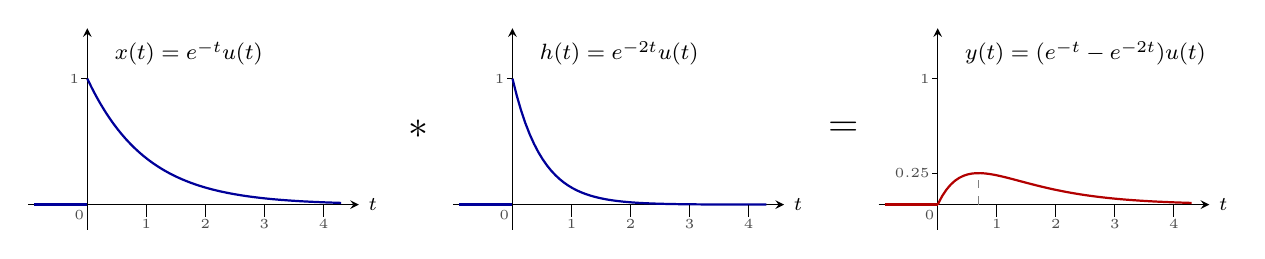
\begin{tikzpicture}[x=0.75cm,y=1.6cm]
  \begin{scope}
    \taxes{-1}{4.6}{1.4}{-0.2}
    \draw[sig] (-0.9,0) -- (0,0);
    \draw[sig,domain=0:4.3,samples=60] plot (\x,{exp(-\x)});
    \foreach \p in {1,2,3,4}{\xt{\p}{\p}}\yt{1}{1}
    \node[anchor=west,font=\footnotesize] at (0.3,1.2) {$x(t)=e^{-t}u(t)$};
  \end{scope}
  \opsym{5.6}{0.6}{$\ast$}
  \begin{scope}[shift={(7.2,0)}]
    \taxes{-1}{4.6}{1.4}{-0.2}
    \draw[sig] (-0.9,0) -- (0,0);
    \draw[sig,domain=0:4.3,samples=60] plot (\x,{exp(-2*\x)});
    \foreach \p in {1,2,3,4}{\xt{\p}{\p}}\yt{1}{1}
    \node[anchor=west,font=\footnotesize] at (0.3,1.2) {$h(t)=e^{-2t}u(t)$};
  \end{scope}
  \opsym{12.8}{0.6}{$=$}
  \begin{scope}[shift={(14.4,0)}]
    \taxes{-1}{4.6}{1.4}{-0.2}
    \draw[res] (-0.9,0) -- (0,0);
    \draw[res,domain=0:4.3,samples=60] plot (\x,{exp(-\x)-exp(-2*\x)});
    \draw[dashed,gray] (0.693,0) -- (0.693,0.25);
    \foreach \p in {1,2,3,4}{\xt{\p}{\p}}\yt{0.25}{0.25}\yt{1}{1}
    \node[anchor=west,font=\footnotesize] at (0.3,1.2) {$y(t)=(e^{-t}-e^{-2t})u(t)$};
  \end{scope}
\end{tikzpicture}
\caption{取 $b=1$、$a=2$ 的例子。结果从 $0$ 开始，先升后降，在 $t=\ln2\approx0.69$ 处达到最大值 $0.25$；没有跳变，与「卷积结果不跳变」一致。}
\end{figure}

\point{代公式。}
\[
x(t)\ast h(t)=\int_{-\infty}^{+\infty}e^{-b\tau}u(\tau)\cdot e^{-a(t-\tau)}u(t-\tau)\,\mathrm{d}\tau .
\]
\textbf{千万不要代错}：$x(\tau)$ 里 $t$ 换成 $\tau$，$h(t-\tau)$ 里 $t$ 换成 $t-\tau$，包括 $u$ 里的自变量。

\point{关键：两个 $u$ 决定积分上下限。}$u(\tau)$ 在 $\tau>0$ 时为 $1$、$\tau<0$ 时为 $0$；$u(t-\tau)$ 在 $\tau<t$ 时为 $1$、$\tau>t$ 时为 $0$。两者相乘，\textbf{只有 $0<\tau<t$ 时 $u(\tau)\,u(t-\tau)=1$}，其他都为 $0$。

\begin{figure}[H]
\centering
\begin{tikzpicture}[x=1.0cm,y=0.9cm]
  \begin{scope}
    \taxes[\tau]{-2}{4.4}{1.6}{-0.2}
    \draw[sig] (-1.9,0) -- (0,0) (0,1) -- (4,1);
    \draw[res,dashed] (-1.9,1.06) -- (2.5,1.06) (2.5,0.03) -- (4,0.03);
    \draw[dotted,red!70!black] (2.5,0) -- (2.5,1.06);
    \fill[green!30,opacity=0.6] (0,0) rectangle (2.5,1);
    \xt{2.5}{t}\xt{-1}{-1}\yt{1}{1}
    \node[anchor=west,font=\scriptsize,blue!60!black] at (3.2,1.3) {$u(\tau)$};
    \node[anchor=east,font=\scriptsize,red!70!black] at (-0.4,1.35) {$u(t-\tau)$};
    \node[font=\scriptsize] at (1.25,0.5) {乘积 $=1$};
    \node[font=\footnotesize] at (1.2,-0.85) {$t>0$：只有 $0<\tau<t$ 时乘积为 $1$};
  \end{scope}
  \begin{scope}[shift={(7.6,0)}]
    \taxes[\tau]{-2}{4.4}{1.6}{-0.2}
    \draw[sig] (-1.9,0) -- (0,0) (0,1) -- (4,1);
    \draw[res,dashed] (-1.9,1.06) -- (-1,1.06) (-1,0.03) -- (4,0.03);
    \draw[dotted,red!70!black] (-1,0) -- (-1,1.06);
    \xt{-1}{t}\xt{2}{2}\yt{1}{1}
    \node[anchor=west,font=\scriptsize,blue!60!black] at (3.2,1.3) {$u(\tau)$};
    \node[font=\footnotesize] at (1.2,-0.85) {$t<0$：两者不重叠，乘积恒为 $0$};
  \end{scope}
\end{tikzpicture}
\caption{蓝：$u(\tau)$，右半边为 $1$；红虚线：$u(t-\tau)$，在 $\tau<t$ 时为 $1$。两者重叠的部分（绿色）就是积分区间 $[0,t]$。}
\end{figure}

\point{分情况。}
\begin{itemize}[nosep]
\item $t<0$：任何 $\tau$ 都使乘积为 $0$，所以 $x(t)\ast h(t)\equiv0$。
\item $t>0$：积分区间变成 $[0,t]$，两个 $u$ 都等于 $1$：
\end{itemize}
\begin{align*}
x(t)\ast h(t)&=\int_0^t e^{-b\tau}e^{-a(t-\tau)}\,\mathrm{d}\tau
=e^{-at}\int_0^t e^{-(b-a)\tau}\,\mathrm{d}\tau\\
&=e^{-at}\cdot\frac{1}{b-a}\Big[1-e^{-(b-a)t}\Big]
=\frac{1}{b-a}\big(e^{-at}-e^{-bt}\big),\qquad t>0 .
\end{align*}

\point{合并成一个式子。}乘 $u(t)$ 就把 $t<0$ 的部分变成 $0$、$t>0$ 的部分保持原样：
\[
x(t)\ast h(t)=\frac{1}{b-a}\big(e^{-at}-e^{-bt}\big)\,u(t).
\]
这个「最后乘 $u(t)$」的技巧很常用。教材写成 $\frac{1}{a-b}\big(e^{-bt}-e^{-at}\big)u(t)$，两者相同。

%==================================================================
\section{图解法}\label{sec:graph}
\example{方波卷直角三角形}{分两段}{教材第 39 页例 2-2}
\textbf{题目}：$x(t)$ 是 $[0,1]$ 上高度为 $1$ 的方波；$h(t)$ 是 $[0,1]$ 上的直角三角形，$t=0$ 处高度为 $1$，直线降到 $t=1$ 处为 $0$。求 $y(t)=x(t)\ast h(t)$。

\point{第一步：取值范围。}最左端 $0+0=0$，最右端 $1+1=2$，所以 $y(t)$ 只在 $[0,2]$ 上有值。

\point{第二步：翻转。}把 $h(\tau)$ 沿纵轴翻转成 $h(-\tau)$：直角边在 $\tau=0$，斜边向左降到 $\tau=-1$。$t=0$ 时，翻转后 $h$ 的最右端正好碰到 $x$ 的最左端，重叠为 $0$。

\point{第三步：平移、相乘、积分。}$h(t-\tau)$ 是把 $h(-\tau)$ 向右移 $t$：它占据 $[t-1,t]$，在 $\tau=t$ 处最高（为 $1$），在 $\tau=t-1$ 处为 $0$。从左往右移动时，先逐渐移进 $x$ 的方波，再逐渐移出，要分两种情况：

\begin{figure}[H]
\centering
\begin{tikzpicture}[x=1.5cm,y=1.5cm]
  \begin{scope}
    \taxes[\tau]{-1.2}{2.3}{1.5}{-0.15}
    \fill[orange!35] (0,0) -- (0,0.4) -- (0.6,1) -- (0.6,0) -- cycle;
    \draw[sig] (0,0) -- (0,1) -- (1,1) -- (1,0);
    \draw[res] (-0.4,0) -- (0.6,1) -- (0.6,0);
    \xt{-0.4}{t-1}\xt{0.6}{t}\xt{1}{1}\xt{2}{2}
    \yt{0.4}{1-t}\yt{1}{1}
    \node[font=\footnotesize] at (0.6,-0.6) {(1) $0<t<1$（图中 $t=0.6$）};
  \end{scope}
  \begin{scope}[shift={(4.0,0)}]
    \taxes[\tau]{-1.2}{2.3}{1.5}{-0.15}
    \fill[orange!35] (0.5,0) -- (1,0.5) -- (1,0) -- cycle;
    \draw[sig] (0,0) -- (0,1) -- (1,1) -- (1,0);
    \draw[res] (0.5,0) -- (1.5,1) -- (1.5,0);
    \xt{0.5}{t-1}\xt{1}{1}\xt{1.5}{t}
    \yt{0.5}{2-t}\yt{1}{1}
    \node[font=\footnotesize] at (0.6,-0.6) {(2) $1<t<2$（图中 $t=1.5$）};
  \end{scope}
\end{tikzpicture}
\caption{蓝：$x(\tau)$；红：$h(t-\tau)$。橙色是两者重叠部分，它的面积就是 $y(t)$（$x$ 的高度为 $1$，乘积就是红线下的面积）。}
\end{figure}

\begin{enumerate}[nosep]
\item $0<t<1$：重叠部分是\textbf{梯形}，底边从 $0$ 到 $t$，长 $t$；左边高 $1-t$（红线在 $\tau=0$ 处的高度），右边高 $1$。
\[
y(t)=\frac{(1-t)+1}{2}\cdot t=\frac{(2-t)\,t}{2}.
\]
\item $1<t<2$：重叠部分是\textbf{三角形}，从 $t-1$ 到 $1$，底边长 $1-(t-1)=2-t$；斜边是 $45^\circ$，高也是 $2-t$。
\[
y(t)=\frac{(2-t)^2}{2}.
\]
\item 其他（$t<0$ 或 $t>2$）：不重叠，$y(t)=0$。
\end{enumerate}

\point{验算：分界点不跳变。}$t=0$：$\frac{(2-0)\cdot0}{2}=0$，与左边的 $0$ 一致。$t=1$：第一段 $\frac{1\cdot1}2=\frac12$，第二段 $\frac{1^2}2=\frac12$，一致。$t=2$：$\frac{0^2}2=0$，与右边的 $0$ 一致。三个分界点都不跳变。

\begin{note}
\textbf{易错点}：第一段的梯形，左边的高是红线在 $\tau=0$ 处的高度 $1-t$，不是 $t$。若误用 $t$，会算成 $\frac{(1+t)t}{2}$，在 $t=1$ 处等于 $1$，与第二段的 $\frac12$ 不连续，用「不跳变」一验就能发现。
\end{note}

\begin{figure}[H]
\centering
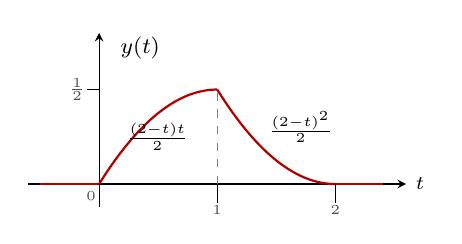
\begin{tikzpicture}[x=1.5cm,y=2.4cm]
  \taxes{-0.6}{2.6}{0.8}{-0.12}
  \draw[res,domain=0:1,samples=40] plot (\x,{(2-\x)*\x/2});
  \draw[res,domain=1:2,samples=40] plot (\x,{(2-\x)^2/2});
  \draw[res] (-0.5,0) -- (0,0) (2,0) -- (2.4,0);
  \draw[dashed,gray] (1,0) -- (1,0.5);
  \xt{1}{1}\xt{2}{2}\yt{0.5}{\frac12}
  \node[anchor=west,font=\scriptsize] at (0.15,0.25) {$\frac{(2-t)t}{2}$};
  \node[anchor=west,font=\scriptsize] at (1.35,0.3) {$\frac{(2-t)^2}{2}$};
  \node[anchor=west,font=\footnotesize] at (0.1,0.72) {$y(t)$};
\end{tikzpicture}
\caption{例 1 的结果：$[0,1]$ 上向上弯地升到 $\frac12$，$[1,2]$ 上向下弯地降到 $0$，处处连续。}
\end{figure}

%==================================================================
\section{两个方波的卷积}\label{sec:rect}
这两个结论要在理解的基础上记住，第三章会用到。

\subsection{宽度相同：三角波}
\begin{remember}
$x(t)$ 是 $[-T_0,T_0]$ 上高度 $E_1$ 的方波，$h(t)$ 是 $[-T_0,T_0]$ 上高度 $E_2$ 的方波，则 $x(t)\ast h(t)$ 是\textbf{三角波}：
\begin{itemize}[nosep]
\item 在 $[-2T_0,2T_0]$ 上有值；
\item 在 $t=0$ 处达到最大值 $2T_0E_1E_2$（重合部分的宽度 $\times$ $x$ 的高度 $\times$ $h$ 的高度）；
\item 两边是直线。
\end{itemize}
\end{remember}

\example{两个 [-1,1] 上的单位方波}{三角波}{}
\textbf{题目}：$x(t)$、$h(t)$ 都是 $[-1,1]$ 上高度为 $1$ 的方波，求 $x(t)\ast h(t)$。

\textbf{解}：
\begin{enumerate}[nosep]
\item 取值范围：最左端 $-1+(-1)=-2$，最右端 $1+1=2$。
\item $t=-2$ 时两个方波刚好碰上，重叠为 $0$。两个方波宽都是 $2$，所以再走 $2$ 个单位（到 $t=0$）时完全重合，达到最大值：宽 $2$ $\times$ 高 $1$ $\times$ 高 $1$ $=2$。
\item 之后再走 $2$ 个单位（到 $t=2$）完全分开，回到 $0$。
\item 移动的距离增加多少，重叠面积就增加（或减少）多少，是线性关系，所以中间都是直线。
\end{enumerate}

\begin{figure}[H]
\centering
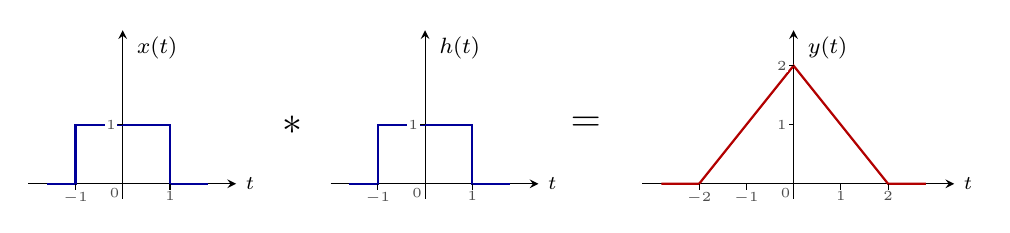
\begin{tikzpicture}[x=0.6cm,y=0.75cm]
  \begin{scope}
    \taxes{-2}{2.4}{2.6}{-0.25}
    \draw[sig] (-1.6,0) -- (-1,0) -- (-1,1) -- (1,1) -- (1,0) -- (1.8,0);
    \xt{-1}{-1}\xt{1}{1}\yt{1}{1}
    \node[anchor=west,font=\footnotesize] at (0.1,2.3) {$x(t)$};
  \end{scope}
  \opsym{3.6}{1}{$\ast$}
  \begin{scope}[shift={(6.4,0)}]
    \taxes{-2}{2.4}{2.6}{-0.25}
    \draw[sig] (-1.6,0) -- (-1,0) -- (-1,1) -- (1,1) -- (1,0) -- (1.8,0);
    \xt{-1}{-1}\xt{1}{1}\yt{1}{1}
    \node[anchor=west,font=\footnotesize] at (0.1,2.3) {$h(t)$};
  \end{scope}
  \opsym{9.8}{1}{$=$}
  \begin{scope}[shift={(14.2,0)}]
    \taxes{-3.2}{3.4}{2.6}{-0.25}
    \draw[res] (-2.8,0) -- (-2,0) -- (0,2) -- (2,0) -- (2.8,0);
    \foreach \p in {-2,-1,1,2}{\xt{\p}{\p}}\yt{1}{1}\yt{2}{2}
    \node[anchor=west,font=\footnotesize] at (0.1,2.3) {$y(t)$};
  \end{scope}
\end{tikzpicture}
\caption{两个宽度都为 $2$ 的单位方波，卷积是 $[-2,2]$ 上的三角波，峰值 $2$。}
\end{figure}

\begin{figure}[H]
\centering
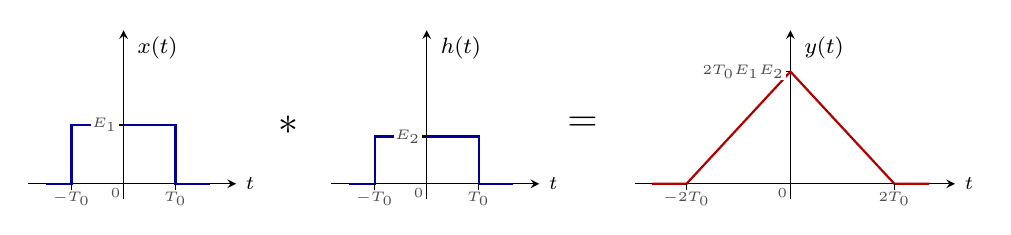
\begin{tikzpicture}[x=0.55cm,y=0.75cm]
  \begin{scope}
    \taxes{-2.2}{2.6}{2.6}{-0.25}
    \draw[sig] (-1.8,0) -- (-1.2,0) -- (-1.2,1) -- (1.2,1) -- (1.2,0) -- (2,0);
    \xt{-1.2}{-T_0}\xt{1.2}{T_0}\yt{1}{E_1}
    \node[anchor=west,font=\footnotesize] at (0.1,2.3) {$x(t)$};
  \end{scope}
  \opsym{3.8}{1}{$\ast$}
  \begin{scope}[shift={(7.0,0)}]
    \taxes{-2.2}{2.6}{2.6}{-0.25}
    \draw[sig] (-1.8,0) -- (-1.2,0) -- (-1.2,0.8) -- (1.2,0.8) -- (1.2,0) -- (2,0);
    \xt{-1.2}{-T_0}\xt{1.2}{T_0}\yt{0.8}{E_2}
    \node[anchor=west,font=\footnotesize] at (0.1,2.3) {$h(t)$};
  \end{scope}
  \opsym{10.6}{1}{$=$}
  \begin{scope}[shift={(15.4,0)}]
    \taxes{-3.6}{3.8}{2.6}{-0.25}
    \draw[res] (-3.2,0) -- (-2.4,0) -- (0,1.9) -- (2.4,0) -- (3.2,0);
    \xt{-2.4}{-2T_0}\xt{2.4}{2T_0}\yt{1.9}{2T_0E_1E_2}
    \node[anchor=west,font=\footnotesize] at (0.1,2.3) {$y(t)$};
  \end{scope}
\end{tikzpicture}
\caption{一般情形：宽度相同（都是 $2T_0$）的两个方波，卷积是 $[-2T_0,2T_0]$ 上的三角波，峰值 $2T_0E_1E_2$。}
\end{figure}

\subsection{宽度不同：梯形波}
\begin{remember}
$x(t)$ 是 $[-A,A]$ 上高度 $E_1$ 的方波，$h(t)$ 是 $[-B,B]$ 上高度 $E_2$ 的方波，$A>B$，则 $x(t)\ast h(t)$ 是\textbf{梯形波}：
\begin{itemize}[nosep]
\item 四个拐点的横坐标：$-A-B,\ \ B-A,\ \ A-B,\ \ A+B$（$B-A$ 与 $A-B$ 互为相反数，梯形左右对称）；
\item 平顶高度 $2BE_1E_2$（\textbf{窄}方波的宽度 $\times$ $E_1$ $\times$ $E_2$）。
\end{itemize}
\end{remember}

\point{四个拐点怎么来。}
\begin{enumerate}[nosep]
\item 起点：$-A-B$（两个最左端相加），两个方波刚好碰上。
\item 窄方波完全移进宽方波，需要再走\textbf{窄方波的宽度} $2B$：$-A-B+2B=B-A$，此后重叠面积达到最大 $2B\cdot E_1E_2$。
\item 窄方波在宽方波里继续走，重叠面积保持不变；能走的距离是\textbf{宽度之差} $2A-2B$：$B-A+(2A-2B)=A-B$。
\item 再走 $2B$ 完全移出：$A-B+2B=A+B$（两个最右端相加）。
\end{enumerate}

\example{[-3,3] 与 [-1,1] 上的单位方波}{梯形波}{}
\textbf{题目}：$x(t)$ 是 $[-3,3]$ 上高度 $1$ 的方波，$h(t)$ 是 $[-1,1]$ 上高度 $1$ 的方波，求 $x(t)\ast h(t)$。

\textbf{解}：$A=3$，$B=1$。起点 $-4$；走窄方波宽度 $2$ 到 $-2$，达到最大值 $2\times1\times1=2$；保持不变走 $6-2=4$ 个单位到 $2$；再走 $2$ 到 $4$ 回到 $0$。

\begin{figure}[H]
\centering
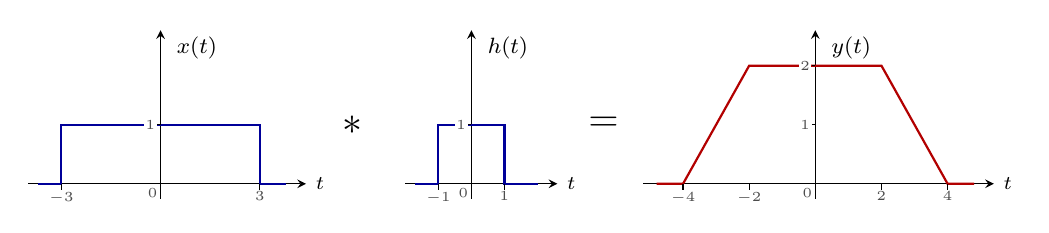
\begin{tikzpicture}[x=0.42cm,y=0.75cm]
  \begin{scope}
    \taxes{-4}{4.4}{2.6}{-0.25}
    \draw[sig] (-3.7,0) -- (-3,0) -- (-3,1) -- (3,1) -- (3,0) -- (3.8,0);
    \xt{-3}{-3}\xt{3}{3}\yt{1}{1}
    \node[anchor=west,font=\footnotesize] at (0.2,2.3) {$x(t)$};
  \end{scope}
  \opsym{5.8}{1}{$\ast$}
  \begin{scope}[shift={(9.4,0)}]
    \taxes{-2}{2.6}{2.6}{-0.25}
    \draw[sig] (-1.7,0) -- (-1,0) -- (-1,1) -- (1,1) -- (1,0) -- (2,0);
    \xt{-1}{-1}\xt{1}{1}\yt{1}{1}
    \node[anchor=west,font=\footnotesize] at (0.2,2.3) {$h(t)$};
  \end{scope}
  \opsym{13.4}{1}{$=$}
  \begin{scope}[shift={(19.8,0)}]
    \taxes{-5.2}{5.4}{2.6}{-0.25}
    \draw[res] (-4.8,0) -- (-4,0) -- (-2,2) -- (2,2) -- (4,0) -- (4.8,0);
    \foreach \p in {-4,-2,2,4}{\xt{\p}{\p}}\yt{1}{1}\yt{2}{2}
    \node[anchor=west,font=\footnotesize] at (0.2,2.3) {$y(t)$};
  \end{scope}
\end{tikzpicture}
\caption{宽度 $6$ 与宽度 $2$ 的单位方波卷积：梯形，拐点 $-4,-2,2,4$，平顶高度 $2$。}
\end{figure}

\begin{figure}[H]
\centering
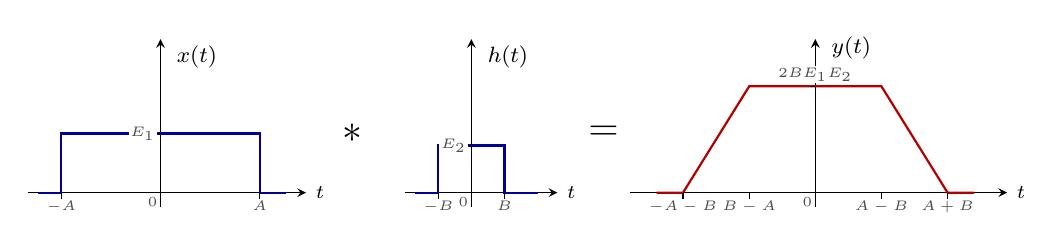
\begin{tikzpicture}[x=0.42cm,y=0.75cm]
  \begin{scope}
    \taxes{-4}{4.4}{2.6}{-0.25}
    \draw[sig] (-3.7,0) -- (-3,0) -- (-3,1) -- (3,1) -- (3,0) -- (3.8,0);
    \xt{-3}{-A}\xt{3}{A}\yt{1}{E_1}
    \node[anchor=west,font=\footnotesize] at (0.2,2.3) {$x(t)$};
  \end{scope}
  \opsym{5.8}{1}{$\ast$}
  \begin{scope}[shift={(9.4,0)}]
    \taxes{-2}{2.6}{2.6}{-0.25}
    \draw[sig] (-1.7,0) -- (-1,0) -- (-1,0.8) -- (1,0.8) -- (1,0) -- (2,0);
    \xt{-1}{-B}\xt{1}{B}\yt{0.8}{E_2}
    \node[anchor=west,font=\footnotesize] at (0.2,2.3) {$h(t)$};
  \end{scope}
  \opsym{13.4}{1}{$=$}
  \begin{scope}[shift={(19.8,0)}]
    \taxes{-5.6}{5.8}{2.6}{-0.25}
    \draw[res] (-4.8,0) -- (-4,0) -- (-2,1.8) -- (2,1.8) -- (4,0) -- (4.8,0);
    \xt{-4}{-A-B}\xt{-2}{B-A}\xt{2}{A-B}\xt{4}{A+B}
    \draw (0,1.8) -- (-0.15,1.8);
    \node[anchor=south,font=\tiny,gray!60!black,fill=white,inner sep=0.6pt] at (0,1.85) {$2BE_1E_2$};
    \node[anchor=west,font=\footnotesize] at (0.2,2.45) {$y(t)$};
  \end{scope}
\end{tikzpicture}
\caption{一般情形（$A>B$）：梯形的四个拐点 $-A-B$、$B-A$、$A-B$、$A+B$，平顶高度 $2BE_1E_2$。}
\end{figure}

\begin{remember}
\textbf{分段为常数的信号卷积，关键点之间连直线}：若 $x(t)$、$h(t)$ 都由若干段方波拼成，算出几个关键点上 $y(t)$ 的值，用直线依次连起来就是答案。原因：两个方波相对移动时，重叠面积随移动距离线性变化。
\end{remember}

%==================================================================
\section{综合例题}\label{sec:ex}
\example{两段台阶卷两段台阶}{关键点连直线}{}
\textbf{题目}：$x(t)$ 在 $[-1,0]$ 上为 $1$、$[0,1]$ 上为 $-2$；$h(t)$ 在 $[-1,0]$ 上为 $1$、$[0,1]$ 上为 $2$。求 $y(t)=x(t)\ast h(t)$。

\textbf{解}：
\begin{enumerate}[nosep]
\item \textbf{取值范围}：最左端 $-1+(-1)=-2$，最右端 $1+1=2$。
\item \textbf{翻转}：$h(-\tau)$ 在 $[-1,0]$ 上为 $2$、$[0,1]$ 上为 $1$（左右对调）。$t=-2$ 时 $h$ 翻转后的最右端碰到 $x$ 的最左端，$y(-2)=0$。
\item \textbf{每移一个单位算一次}（各段宽度都是 $1$，关键点在整数处）：
  \begin{itemize}[nosep]
  \item $t=-1$：$h$ 的「$1$」那段与 $x$ 的「$1$」那段重合，$y(-1)=1\times1\times1=1$。
  \item $t=0$：$h$ 的「$2$」对 $x$ 的「$1$」、$h$ 的「$1$」对 $x$ 的「$-2$」，$y(0)=2\times1\times1+(-2)\times1\times1=0$。
  \item $t=1$：只剩 $h$ 的「$2$」对 $x$ 的「$-2$」，$y(1)=(-2)\times2\times1=-4$。
  \item $t=2$：完全移出，$y(2)=0$。
  \end{itemize}
\item 关键点之间连直线。
\end{enumerate}

\begin{figure}[H]
\centering
\begin{tikzpicture}[x=0.75cm,y=0.5cm]
  \begin{scope}
    \taxes{-1.8}{1.9}{2.6}{-2.6}
    \draw[sig] (-1.5,0) -- (-1,0) -- (-1,1) -- (0,1) -- (0,-2) -- (1,-2) -- (1,0) -- (1.5,0);
    \xtu{-1}{-1}\xtu{1}{1}\yt{1}{1}
    \draw (0,-2) -- (-0.1,-2) node[anchor=east,font=\tiny,gray!60!black,fill=white,inner sep=0.6pt] {$-2$};
    \node[anchor=west,font=\footnotesize] at (0.15,2.3) {$x(t)$};
  \end{scope}
  \opsym{3.0}{0}{$\ast$}
  \begin{scope}[shift={(5.4,0)}]
    \taxes{-1.8}{1.9}{2.6}{-2.6}
    \draw[sig] (-1.5,0) -- (-1,0) -- (-1,1) -- (0,1) -- (0,2) -- (1,2) -- (1,0) -- (1.5,0);
    \xt{-1}{-1}\xt{1}{1}\yt{1}{1}\yt{2}{2}
    \node[anchor=west,font=\footnotesize] at (1.1,2.3) {$h(t)$};
  \end{scope}
  \opsym{8.0}{0}{$=$}
  \begin{scope}[shift={(11.6,0)}]
    \taxes{-2.8}{2.9}{2.6}{-4.6}
    \draw[res] (-2.6,0) -- (-2,0) -- (-1,1) -- (0,0) -- (1,-4) -- (2,0) -- (2.6,0);
    \foreach \p/\v in {-2/0,-1/1,0/0,1/-4,2/0}{\fill[red!70!black] (\p,\v) circle (1.6pt);}
    \xtu{-2}{-2}\xt{-1}{-1}\xtu{1}{1}\xtu{2}{2}
    \yt{1}{1}
    \draw (0,-4) -- (-0.1,-4) node[anchor=east,font=\tiny,gray!60!black,fill=white,inner sep=0.6pt] {$-4$};
    \node[anchor=west,font=\footnotesize] at (0.15,2.3) {$y(t)$};
  \end{scope}
\end{tikzpicture}
\caption{结果是 $(-2,0)$、$(-1,1)$、$(0,0)$、$(1,-4)$、$(2,0)$ 五个关键点依次连成的折线。}
\end{figure}

\example{方波卷两段台阶}{关键点连直线}{教材第 78 页图 2-44 第二个}
\textbf{题目}：$x(t)$ 是 $[-1,0]$ 上高度 $1$ 的方波；$h(t)$ 在 $[-1,0]$ 上为 $1$、$[0,1]$ 上为 $2$。求 $x(t)\ast h(t)$。

\textbf{解}：取值范围 $[-2,1]$。$x$ 是宽度 $1$ 的单位方波，所以 $y(t)$ 等于 $h$ 在长度为 $1$ 的窗口 $[t,t+1]$ 上的积分：$y(-2)=0$，$y(-1)=\int_{-1}^0h=1$，$y(0)=\int_0^1h=2$，$y(1)=0$。关键点连直线。

\begin{figure}[H]
\centering
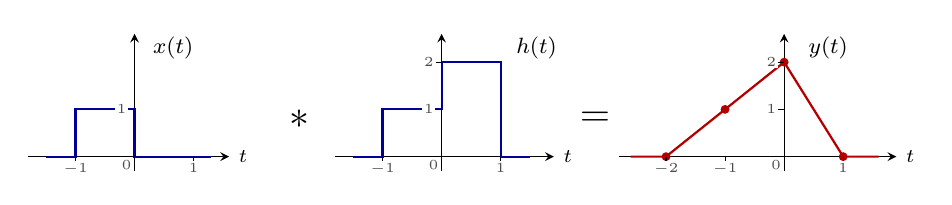
\begin{tikzpicture}[x=0.75cm,y=0.6cm]
  \begin{scope}
    \taxes{-1.8}{1.6}{2.6}{-0.3}
    \draw[sig] (-1.5,0) -- (-1,0) -- (-1,1) -- (0,1) -- (0,0) -- (1.3,0);
    \xt{-1}{-1}\xt{1}{1}\yt{1}{1}
    \node[anchor=west,font=\footnotesize] at (0.15,2.3) {$x(t)$};
  \end{scope}
  \opsym{2.8}{0.8}{$\ast$}
  \begin{scope}[shift={(5.2,0)}]
    \taxes{-1.8}{1.9}{2.6}{-0.3}
    \draw[sig] (-1.5,0) -- (-1,0) -- (-1,1) -- (0,1) -- (0,2) -- (1,2) -- (1,0) -- (1.5,0);
    \xt{-1}{-1}\xt{1}{1}\yt{1}{1}\yt{2}{2}
    \node[anchor=west,font=\footnotesize] at (1.1,2.3) {$h(t)$};
  \end{scope}
  \opsym{7.8}{0.8}{$=$}
  \begin{scope}[shift={(11.0,0)}]
    \taxes{-2.8}{1.9}{2.6}{-0.3}
    \draw[res] (-2.6,0) -- (-2,0) -- (-1,1) -- (0,2) -- (1,0) -- (1.6,0);
    \foreach \p/\v in {-2/0,-1/1,0/2,1/0}{\fill[red!70!black] (\p,\v) circle (1.6pt);}
    \xt{-2}{-2}\xt{-1}{-1}\xt{1}{1}\yt{1}{1}\yt{2}{2}
    \node[anchor=west,font=\footnotesize] at (0.25,2.3) {$y(t)$};
  \end{scope}
\end{tikzpicture}
\caption{结果是 $(-2,0)$、$(-1,1)$、$(0,2)$、$(1,0)$ 连成的折线。}
\end{figure}

\example{周期方波卷三角波}{周期为 2}{教材第 78 页图 2-44 最下面一个}
\textbf{题目}：$x(t)$ 是周期为 $2$ 的方波：在 $(0,1)$ 上为 $1$、$(1,2)$ 上为 $-1$，向两边无限重复。$h(t)$ 是 $[0,2]$ 上的三角波，$t=1$ 处峰值为 $1$。求 $y(t)=x(t)\ast h(t)$。

\point{先看结构。}$x$ 从 $-\infty$ 延伸到 $+\infty$，所以 $y$ 也是。$x$ 以 $2$ 为周期重复，$h$ 每移 $2$ 个单位看到的情况完全一样，所以 \textbf{$y(t)$ 也是周期为 $2$ 的函数}，只需求出一个周期 $[0,2]$。

\point{$t=0$。}翻转后的三角形占据 $[-2,0]$，左半边落在 $x=1$ 的 $(-2,-1)$ 上，右半边落在 $x=-1$ 的 $(-1,0)$ 上；两半面积相同，正负抵消，$y(0)=0$。

\point{$0<t<1$。}三角形 $h(t-\tau)$ 占据 $[t-2,t]$，峰在 $\tau=t-1$。它被 $x$ 的跳变点 $\tau=-1$、$\tau=0$ 分成三块：

\begin{figure}[H]
\centering
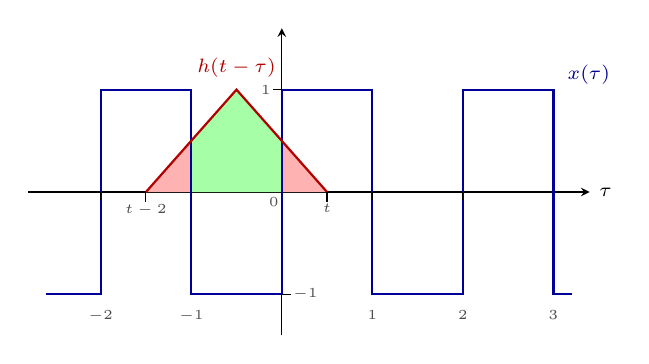
\begin{tikzpicture}[x=1.15cm,y=1.3cm]
  \taxes[\tau]{-2.8}{3.4}{1.6}{-1.4}
  \fill[red!30] (-1.5,0) -- (-1,0.5) -- (-1,0) -- cycle;
  \fill[green!35] (-1,0) -- (-1,0.5) -- (-0.5,1) -- (0,0.5) -- (0,0) -- cycle;
  \fill[red!30] (0,0) -- (0,0.5) -- (0.5,0) -- cycle;
  \draw[sig] (-2.6,-1) -- (-2,-1) -- (-2,1) -- (-1,1) -- (-1,-1) -- (0,-1) -- (0,1) -- (1,1) -- (1,-1) -- (2,-1) -- (2,1) -- (3,1) -- (3,-1) -- (3.2,-1);
  \draw[res] (-1.5,0) -- (-0.5,1) -- (0.5,0);
  \foreach \p in {-2,-1,1,2,3}{\draw (\p,0) -- (\p,-0.08); \node[anchor=north,font=\tiny,gray!60!black] at (\p,-1.06) {$\p$};}
  \xt{-1.5}{t-2}\xt{0.5}{t}
  \yt{1}{1}
  \draw (0,-1) -- (0.1,-1) node[anchor=west,font=\tiny,gray!60!black,fill=white,inner sep=0.6pt] {$-1$};
  \node[anchor=west,font=\scriptsize,blue!60!black] at (3.05,1.15) {$x(\tau)$};
  \node[anchor=south,font=\scriptsize,red!70!black] at (-0.5,1.02) {$h(t-\tau)$};
\end{tikzpicture}
\caption{$0<t<1$（图中 $t=0.5$）：两块红色落在 $x=+1$ 上，乘 $+1$；绿色落在 $x=-1$ 上，乘 $-1$。横轴刻度数字标在方波下沿下方。所以 $y(t)=$ 两块红色面积 $-$ 绿色面积。}
\end{figure}

\begin{itemize}[nosep]
\item 右边红色：$\tau\in[0,t]$，是腰长 $t$ 的等腰直角三角形，面积 $\frac{t^2}2$；
\item 左边红色：$\tau\in[t-2,-1]$，底边长 $-1-(t-2)=1-t$，面积 $\frac{(1-t)^2}2$；
\item 绿色：整个三角形面积 $\frac{2\times1}2=1$ 减去两块红色：$1-\frac{t^2}2-\frac{(1-t)^2}2$。
\end{itemize}
\[
y(t)=\frac{t^2}2+\frac{(1-t)^2}2-\Big[1-\frac{t^2}2-\frac{(1-t)^2}2\Big]=t^2+(1-t)^2-1,\qquad 0<t<1 .
\]
验算：$t=0$ 时 $0+1-1=0$，与 $y(0)=0$ 一致。

\point{$1<t<2$。}三角形占据 $[t-2,t]$，被 $\tau=0$、$\tau=1$ 分成三块：中间一块落在 $x=+1$ 的 $(0,1)$ 上，两边两块落在 $x=-1$ 上。
\begin{itemize}[nosep]
\item 右边：$\tau\in[1,t]$，面积 $\frac{(t-1)^2}2$；
\item 左边：$\tau\in[t-2,0]$，底边长 $2-t$，面积 $\frac{(2-t)^2}2$；
\item 中间：$1-\frac{(t-1)^2}2-\frac{(2-t)^2}2$。
\end{itemize}
\[
y(t)=\Big[1-\frac{(t-1)^2}2-\frac{(t-2)^2}2\Big]-\frac{(t-1)^2}2-\frac{(t-2)^2}2=1-(t-1)^2-(t-2)^2,\qquad 1<t<2 .
\]
验算：$t=1$ 时第一段 $1+0-1=0$，第二段 $1-0-1=0$，不跳变。

\point{化简与图形。}第一段 $=2t^2-2t=-2t(1-t)$，在 $t=\frac12$ 处最小为 $-\frac12$；第二段 $=-2(t-1)(t-2)$，在 $t=\frac32$ 处最大为 $\frac12$。再以 $2$ 为周期重复。

\begin{figure}[H]
\centering
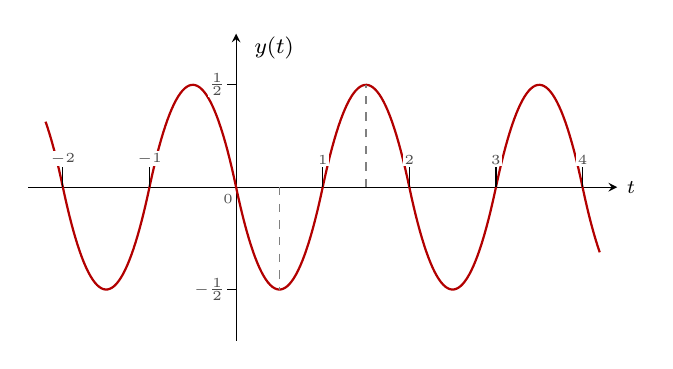
\begin{tikzpicture}[x=1.1cm,y=2.6cm]
  \taxes{-2.4}{4.4}{0.75}{-0.75}
  \draw[res,domain=-2.2:4.2,samples=260] plot (\x,{(mod(\x+10,2)<1) ? (2*mod(\x+10,2)^2-2*mod(\x+10,2)) : (-2*mod(\x+10,2)^2+6*mod(\x+10,2)-4)});
  \foreach \p in {-2,-1,1,2,3,4}{\xtu{\p}{\p}}
  \yt{0.5}{\frac12}
  \draw (0,-0.5) -- (-0.1,-0.5) node[anchor=east,font=\tiny,gray!60!black,fill=white,inner sep=0.6pt] {$-\frac12$};
  \draw[dashed,gray] (0.5,0) -- (0.5,-0.5) (1.5,0) -- (1.5,0.5);
  \node[anchor=west,font=\footnotesize] at (0.1,0.68) {$y(t)$};
\end{tikzpicture}
\caption{$y(t)$：$(0,1)$ 上是向下的抛物线拱（最低 $-\frac12$），$(1,2)$ 上是向上的抛物线拱（最高 $\frac12$），以 $2$ 为周期重复。}
\end{figure}

%==================================================================
\section{冲激的尺度变换：易错题}\label{sec:delta}
\begin{remember}
\[
\delta(at)=\frac1{|a|}\,\delta(t),\qquad
\delta(at+b)=\frac1{|a|}\,\delta\!\left(t+\frac ba\right).
\]
冲激的性质与普通信号相反：\textbf{波形拉伸 $k$ 倍时，冲激的强度变为 $k$ 倍；压缩 $k$ 倍时，强度变为 $\frac1k$}。第五章还会用到这一点。
\end{remember}

\example{已知 x(3-2t) 的波形，求 x(t)}{冲激强度变为 4}{教材第 31 页 1-9}
\textbf{题目}：$x(3-2t)$ 的波形是：$t=1$ 处一个 $2$ 倍的冲激 $2\delta(t-1)$，$[2,3]$ 上为 $1$，$[3,4]$ 上为 $2$。求 $x(t)$。

\point{换元。}设 $t'=3-2t$，则 $t=\frac{3-t'}2$，所以 $x(t')$ 就是已知波形在 $\frac{3-t'}2$ 处的值。把 $t'$ 改写回 $t$，要求的是已知波形 $g(t)=x(3-2t)$ 变换成
\[
x(t)=g\!\left(\frac{3-t}2\right)=g\!\left(-\frac12(t-3)\right).
\]

\point{三步变换。}
\begin{enumerate}[nosep]
\item \textbf{翻转}（前面有负号）：$g(-t)$。冲激移到 $-1$；台阶变成 $[-3,-2]$ 上为 $1$、$[-4,-3]$ 上为 $2$。
\item \textbf{拉伸}（系数 $\left|-\frac12\right|<1$，拉伸 $2$ 倍）：$g\!\left(-\frac t2\right)$。冲激移到 $-2$；台阶变成 $[-6,-4]$ 上为 $1$、$[-8,-6]$ 上为 $2$。
\item \textbf{右移 $3$}（$t-3$）：冲激移到 $1$；台阶变成 $[-3,-1]$ 上为 $1$、$[-5,-3]$ 上为 $2$。
\end{enumerate}

\point{易错点：冲激的强度。}台阶的高度在变换中不变，但冲激的强度会变。单独算冲激这一项：
\begin{align*}
2\,\delta\!\left(\frac{3-t}2-1\right)
&=2\,\delta\!\left(-\frac12t+\frac12\right)
=2\,\delta\!\left(-\frac12(t-1)\right)\\
&=2\cdot\frac{1}{\left|-\frac12\right|}\,\delta(t-1)=4\,\delta(t-1).
\end{align*}
所以拉伸那一步，冲激的强度从 $2$ 变成 $4$。若照搬台阶的做法保持强度 $2$，答案就错了。

\begin{remember}
\textbf{答案}：$x(t)=4\,\delta(t-1)$，加上 $[-5,-3]$ 上为 $2$、$[-3,-1]$ 上为 $1$ 的台阶。
\end{remember}

\begin{figure}[H]
\centering
\begin{tikzpicture}[x=0.42cm,y=0.42cm]
  \begin{scope}
    \taxes{-8.8}{4.8}{4.8}{-0.4}
    \draw[sig] (2,0) -- (2,1) -- (3,1) -- (3,2) -- (4,2) -- (4,0);
    \imp{1}{2.4}{$(2)$}
    \foreach \p in {1,2,3,4}{\xt{\p}{\p}}\yt{1}{1}\yt{2}{2}
    \node[anchor=west,font=\footnotesize] at (-8.6,4.2) {已知 $g(t)=x(3-2t)$};
  \end{scope}
  \begin{scope}[shift={(15.5,0)}]
    \taxes{-8.8}{4.8}{4.8}{-0.4}
    \draw[sig] (-4,0) -- (-4,2) -- (-3,2) -- (-3,1) -- (-2,1) -- (-2,0);
    \imp{-1}{2.4}{$(2)$}
    \foreach \p in {-4,-3,-2}{\xt{\p}{\p}}\xt{1}{1}\yt{1}{1}\yt{2}{2}
    \node[anchor=west,font=\footnotesize] at (-8.6,4.2) {(1) 翻转 $g(-t)$};
  \end{scope}
  \begin{scope}[shift={(0,-8)}]
    \taxes{-8.8}{4.8}{4.8}{-0.4}
    \draw[sig] (-8,0) -- (-8,2) -- (-6,2) -- (-6,1) -- (-4,1) -- (-4,0);
    \imp{-2}{4}{$(4)$}
    \foreach \p in {-8,-6,-4,-2}{\xt{\p}{\p}}\xt{2}{2}\yt{1}{1}\yt{2}{2}
    \node[anchor=west,font=\footnotesize] at (-8.6,4.2) {(2) 拉伸 $g(-\frac t2)$};
  \end{scope}
  \begin{scope}[shift={(15.5,-8)}]
    \taxes{-8.8}{4.8}{4.8}{-0.4}
    \draw[sig] (-5,0) -- (-5,2) -- (-3,2) -- (-3,1) -- (-1,1) -- (-1,0);
    \imp{1}{4}{$(4)$}
    \foreach \p in {-5,-3,-1,1}{\xt{\p}{\p}}\xt{3}{3}\yt{1}{1}\yt{2}{2}
    \node[anchor=west,font=\footnotesize] at (-8.6,4.2) {(3) 右移 3：$x(t)$};
  \end{scope}
\end{tikzpicture}
\caption{由 $x(3-2t)$ 求 $x(t)$ 的三步。台阶高度不变；冲激（括号里是强度）在拉伸 $2$ 倍时强度由 $2$ 变成 $4$。}
\end{figure}

\end{document}
